\section{Introduction}

We consider the incompressible Euler equations in the plane, in vorticity form:
\begin{equation}
\label{eq:euler}
\partial_t \omega + v\cdot\nabla \omega = 0,\qquad
v = \KBS\ast \omega,\qquad
\omega(t=0) = \omega_0 .
\end{equation}
Here $\KBS(x)=x^\perp/(2\pi|x|^2)$, $x^\perp=(-x_2,x_1)$, denotes the
Biot-Savart kernel, so that $v$ is divergence free and
$\partial_1v_2-\partial_2v_1=\omega$. There is no external force, and we call
$\omega_0$ the datum.

For a smooth decaying datum, Equation~\eqref{eq:euler} has a unique global
smooth solution (Wolibner \cite{Wolibner}, H\"older \cite{Holder}; see Kato
\cite{Kato1967}; a self-contained proof for compactly supported data is in
Appendix~B of Part~II~\cite{PartII}). Yudovich proved in \cite{Yudovich1963}, for
bounded domains, that a weak solution with bounded vorticity is unique: its
velocity is log-Lipschitz, which closes an energy estimate for the difference of
two solutions. For the
plane, with vorticity in $(L^1\cap L^\infty)(\R^2)$ and square-integrable
velocity, a complete proof is given in Theorem~0.3 and Appendix~B.2 of \cite{ABCDGJK}.
For a datum in $(L^1\cap L^p)(\Omega)$, $1<p<\infty$, global weak solutions exist
(Yudovich for a bounded domain $\Omega$ \cite{Yudovich1963}, see the introduction of
\cite{Yudovich1995}; DiPerna and Majda for $\Omega=\R^2$ \cite{DiPernaMajda}). When $p>4/3$ the product $v\,\omega$ is
locally integrable and Equation~\eqref{eq:euler} has a weak formulation
(Lemma~\ref{lem:velocity}, Definition~\ref{def:weak}), but the velocity is only
Sobolev regular and Yudovich's uniqueness argument does not apply. Whether his theorem
extends to vorticity in $L^\infty_tL^p_x$, $p<\infty$, is the question of
Section~1.1.1 of \cite{BrueColomboKumar}. This paper and Part~II~\cite{PartII} prove that, without force in the
plane, uniqueness fails among renormalized weak solutions with vorticity in
$L^\infty_t(L^1\cap L^q)_x$, for every $q\in(4/3,\infty)$ at once and for an
explicit radial datum. The velocity of our datum is not square integrable (see
below), whereas the planar theorem of \cite{ABCDGJK} assumes
it is, and the question of \cite{BrueColomboKumar} is posed on $\mathbb T^2$.

Uniqueness is known in several classes of unbounded vorticity. Yudovich proved
in Theorem~1 of \cite{Yudovich1995}, in a bounded domain $D$, uniqueness among
solutions whose vorticity lies in every $L^p(D)$ with $p<\infty$, with $\|\omega(t)\|_{L^p(D)}$ bounded, for all large $p$, by a constant
multiple of a growth function of $p$ satisfying a divergence condition of Osgood
type. Taniuchi introduced uniformly local versions of these spaces on $\R^2$
and constructed global solutions in them \cite{Taniuchi}; uniqueness there
under the same kind of divergence condition is proved by Chen, Miao and Zheng
\cite{ChenMiaoZheng} and stated as Theorem~1.4 of \cite{CrippaStefani}, both
crediting Taniuchi, and Crippa and Stefani gave a Lagrangian proof of
uniqueness in localized Yudovich spaces (Theorem~1.6 of \cite{CrippaStefani}).
Vishik proved uniqueness in Besov-type spaces containing the local space $\mathrm{bmo}$, under an
additional integrability condition \cite{Vishik1999}. Bernicot and Keraani
\cite{BernicotKeraani}, Bernicot and Hmidi \cite{BernicotHmidi}, and Chen, Miao
and Zheng \cite{ChenMiaoZheng} gave spaces of unbounded vorticity with global
existence, uniqueness or propagation of the class; Elgindi, Murray and Said
\cite{ElgindiMurraySaid} gave a local-in-time existence and uniqueness class
whose solutions can leave it in finite time. Our datum satisfies none of these
uniqueness criteria: its $L^p(\R^2)$ norms grow exponentially in $p$, it is not in
$\mathrm{BMO}$, its dyadic blocks grow too fast for the spaces of
\cite{Vishik1999}, and it is not odd in the angle. We leave the verification of
these facts to the interested reader. So Theorem~\ref{thm:main} contradicts
none of these results.

With a radial force, Vishik \cite{Vishik1}, \cite{Vishik2} proved
non-uniqueness with vorticity in an $L^p(\R^2)$ space, breaking the radial symmetry. In the
account of Albritton, Bru\`e, Colombo, De Lellis, Giri, Janisch and Kwon
\cite{ABCDGJK}, for every $p\in(2,\infty)$ there are a datum in $(L^1\cap L^p)(\R^2)$
(possibly zero) with velocity in $L^2(\R^2)$ and a force in $L^1_t(L^1\cap L^p)_x$ whose
Biot-Savart velocity lies in $L^1_tL^2_x$, with uncountably many solutions with vorticity in
$L^\infty_t(L^1\cap L^p)_x$ and velocity in $L^\infty_tL^2_x$. The unstable
manifold of a steady vortex gives non-uniqueness only at time $-\infty$;
Vishik's self-similar background moves time $-\infty$ to time $0$, but it is
not an exact solution and requires the force (Section~0.1 of \cite{ABCDGJK}).
Without force, convex integration gives non-uniqueness for vorticity in $L^p(\R^2)$ and
$L^p(\mathbb T^2)$:
Mengual \cite{Mengual} showed, for $2<p<\infty$, that a truncated power-law
vortex, a steady solution with vorticity in $(L^1\cap L^p)(\R^2)$, is the datum of
infinitely many bounded admissible weak solutions, with velocity in $C_tL^2_x$.
In that result only the initial vorticity lies in $L^p$: at positive times the
vorticity of these solutions is known only as a distribution inside a growing disk,
so they are not known to lie in the class $L^\infty_tL^p_x$ of the question above.
Both solutions of Theorem~\ref{thm:main}, in contrast, have vorticity in
$L^\infty_t(L^1\cap L^q)_x$ for every $q\in(4/3,\infty)$, so Theorem~\ref{thm:main}
answers that question in the plane, in the class in which it is posed. Bru\`e,
Colombo and Kumar (Theorem~1.2 of \cite{BrueColomboKumar}) obtained, on
$\mathbb T^2$, for some $p>1$ and a dense set of initial velocities, infinitely
many weak solutions with vorticity in $C([0,1];L^p(\mathbb T^2))$, which do not conserve
energy. Outside the $L^p$ scale, convex integration also gives unforced
non-uniqueness: \cite{BrueColombo}
($L^{1,\infty}$ vorticity, bounded energy) and \cite{BuckModena} (Hardy spaces
$H^p(\R^2)$, $2/3<p<1$).

In an instability construction without force, the background must be an exact
solution. Ours is radial, hence stationary: infinitely many rescaled copies of
one unstable vortex ring on disjoint annuli accumulating at the origin, with
amplitudes increasing toward it. Inner rings rotate faster, and the task is to
carry an instability from an inner ring outward through every ring in a time
independent of the depth, uniformly in the number of interacting rings.

For $T>0$ and $1\le q\le\infty$ we write $X_q(T)$ for the space
$L^\infty_t(L^1\cap L^q)_x$ of functions on $(0,T)\times\R^2$. Renormalized weak solutions in $X_q(T)$, $q>4/3$ (after
DiPerna and Lions \cite{DiPernaLions}), and equimeasurability are defined in
Definitions~\ref{def:weak} and~\ref{def:equimeasurable}. The ring $\Phi$ of
Definition~\ref{def:ring} is a closed formula in $\log|y|$ times a fixed smooth
cutoff; it is radial, $\Phi\in C_c^\infty(\R^2)$, $0\le\Phi<1$,
$\Phi\not\equiv0$, and $\supp\Phi\subset\{a\le|y|\le1\}$ for an explicit
$a\in(0,1)$ (Lemma~\ref{lem:ring-facts}). For $A_1>0$, $\mu\in(1,2]$ and
$\sbar\in(0,a/16]$ we put
\begin{equation}
\label{eq:datum}
\begin{gathered}
f=\sum_{k\ge1}A_k\,\Phi(\cdot/r_k),\qquad A_k=A_1\mu^{k-1},\\
r_1=1,\qquad r_{k+1}=s_kr_k,\qquad s_k=\sbar(2\mu)^{-k}\qquad(k\ge1).
\end{gathered}
\end{equation}
The main theorem of the two papers is the following.

\begin{theorem}
\label{thm:main}
Let $\Phi$ and $a$ be as in Definition~\ref{def:ring}. There are
$\mu\in(1,\frac{17}{16}]$ and $\sbar\in(0,a/16]$ such that, for every $A_1>0$,
the function $f$ of Equation~\eqref{eq:datum} has the following properties. It
is radial and nonnegative, $f\in (L^1\cap L^q)(\R^2)$ for every $q\in[1,\infty)$,
and $f\notin L^\infty(\R^2)$. There is $\Tstar\in(0,\infty)$ such that, for
every $T>\Tstar$ and every $q\in(4/3,\infty)$, Equation~\eqref{eq:euler} with
$\omega_0=f$ has two distinct renormalized weak solutions in $X_q(T)$, in the
sense of Definition~\ref{def:weak}:
\begin{enumerate}[label=\textup{(\roman*)}]
\item the stationary solution $\omega(t)=f$, $t\in[0,T]$;
\item a solution $\omega_\infty$ such that
  $\omega_\infty\in C([0,\infty);L^p(\R^2))$ for every $p\in[1,\infty)$ and,
  for every $t\ge0$, $\omega_\infty(t)$ is equimeasurable with $f$ and
  $3$-fold rotationally symmetric.
\end{enumerate}
More precisely, there is $t_0\in[0,\Tstar)$ such that $\omega_\infty$ and $f$
are distinct elements of $X_q(T')$ for every $T'>t_0$ and every
$q\in(4/3,\infty)$.
\end{theorem}

We do not treat $q\le4/3$. No symmetry is
imposed on the class; the $3$-fold rotational symmetry of $\omega_\infty$ comes from the
construction, where it removes the angular modes $\ell\notin3\Z$, among them the
modes $\ell=\pm1$ that contain the translations of a ring, and leaves the
modes $\ell\in3\Z$, whose spectra we control under Hypothesis~\ref{hyp:N}.

Theorem~\ref{thm:main} concerns one explicit family of data. It says nothing about the kinetic
energy or the vanishing viscosity limit. The velocity of $f$ is not square integrable: by
Lemma~\ref{lem:radial-stationary}, since $\supp f$ lies in the closed unit disk,
$|\KBS\ast f(x)|=(2\pi|x|)^{-1}\int f$ for almost every $x$ with $|x|\ge1$, and
$\int f>0$.

The proof of Theorem~\ref{thm:main} is divided between this paper and
Part~II~\cite{PartII}. This paper proves a non-uniqueness criterion
(Section~\ref{sec:compact}) and the linear analysis of the ring
(Section~\ref{sec:ring}), and it uses no machine computation. Part~II proves
that \textup{(N1)}--\textup{(N3)} of Hypothesis~\ref{hyp:N} imply
Theorem~\ref{thm:main} (Proposition~1.2 there), by a nonlinear construction
followed by the criterion of Section~\ref{sec:compact}, and it proves
\textup{(N1)}--\textup{(N3)} (Theorem~1.3 there): \textup{(N1)} and
\textup{(N2)} with rigorous interval arithmetic and \textup{(N3)} by hand, in
its Appendix~A. Its Appendix~B gives the existence theory for the global smooth solutions
that the proof uses.

Section~\ref{sec:compact} follows the compactness theory of DiPerna and Lions for
sequences of renormalized solutions, in a self-contained form for vorticity in
$L^\infty_t(L^1\cap L^2)_x$, and proves a compactness criterion for
non-uniqueness (Theorem~\ref{thm:criterion}). The form of it that Part~II uses is
the following conditional non-uniqueness theorem (Corollary~\ref{cor:defect} and
Remark~\ref{rem:conditional}).

\begin{theorem}[Conditional non-uniqueness]
\label{thm:conditional}
Let $f$ be radial with $f\in (L^1\cap L^q)(\R^2)$ for every $q\in[1,\infty)$.
Suppose that there are data $f^{(n)}\to f$ in $(L^1\cap L^2)(\R^2)$ and, for each
$n$, a $3$-fold rotationally symmetric renormalized weak solution $\omega^{(n)}$ of
Equation~\eqref{eq:euler} on $[0,\infty)$ with datum $f^{(n)}$ and vorticity in
$L^\infty_t(L^1\cap L^2)_x$, with the following property: for some integer
$m\ge1$, some real $\chi\in C_c^\infty((0,\infty))$, some $c_0>0$ and
$\bar T\in(0,\infty)$, and some times $T^{(n)}\in[0,\bar T]$,
\[
\Big|\int_{\R^2}\omega^{(n)}(T^{(n)},x)\,\chi(|x|)\,(\bar x)^m\dd x\Big|\ge c_0
\qquad\text{for all large }n,
\]
with $x$ written as a complex number. Then Equation~\eqref{eq:euler} with
$\omega_0=f$ has, besides the stationary solution $\omega(t)=f$, a renormalized
weak solution $\omega_\infty$ with vorticity in $L^\infty_t(L^1\cap L^2)_x$ that is
$3$-fold rotationally symmetric and equimeasurable with $f$ at every time and lies
in $C([0,\infty);L^q(\R^2))$ for every $q\in[1,\infty)$. For some
$t_0\in[0,\bar T)$, $\omega_\infty$ and $f$ are distinct elements of $X_q(T')$ for
every $T'>t_0$ and every $q\in(4/3,\infty)$.
\end{theorem}

Since the moment in Theorem~\ref{thm:conditional} vanishes for the radial
function $f$, its hypothesis says that the approximate solutions leave $f$ by a
fixed amount, in one non-radial moment, within a time bounded independently of
$n$. The second solution is a limit of a subsequence of the $\omega^{(n)}$.

For the datum $f$ of Theorem~\ref{thm:main}, Part~II takes for $f^{(n)}$ the partial
sum of the first $n$ rings of $f$, with the innermost ring replaced by a seeded
ring: a $3$-fold rotationally symmetric copy of $\Phi$, equimeasurable with it and
close to it, that carries a small component along the unstable eigenfunction of
Theorem~\ref{thm:linear} below. Figure~\ref{fig:datum} shows, for $n=10$, the
partial sum $f_{10}=\sum_{k=1}^{10}A_k\Phi(\cdot/r_k)$ of the actual datum $f$ from
which non-uniqueness occurs; $f^{(10)}$ differs from it only by the seed, which is
invisible at this scale.

\begin{figure}[ht]
\centering
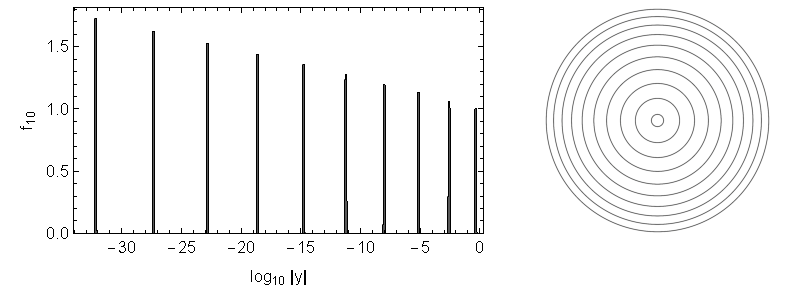
\includegraphics[width=0.95\textwidth]{figures/datum.pdf}
\caption[The partial sum of ten rings of the datum]{The partial sum $f_{10}=\sum_{k=1}^{10}A_k\Phi(\cdot/r_k)$ of the datum $f$ of
Equation~\eqref{eq:datum}, for the illustrative values $A_1=1$, $\mu=\frac{17}{16}$ and
$\sbar=a/16$ (Theorem~\ref{thm:main} uses some $\mu\in(1,\frac{17}{16}]$ and
$\sbar\in(0,a/16]$ that are not computed; a smaller $\sbar$ separates the scales
further), and for the function $\chi$ constructed in the proof of
Lemma~\ref{lem:ring-facts}. Left: $f_{10}$ against $\log_{10}|y|$; the rings sit at
the scales $r_1=1>r_2>\dots>r_{10}\approx10^{-32}$, and their amplitudes
$A_k=\mu^{k-1}$ grow toward the origin. Right: the same ten rings in a logarithmic
polar picture, in which the distance from the center is an affine function of
$\log|y|$, so that all of them are visible; each ring is drawn without its amplitude,
darker where $\Phi(\cdot/r_k)$ is larger. Drawn with Mathematica from the exact
formulas; the figure is an illustration and is not used in any proof.}
\label{fig:datum}
\end{figure}

The proof of Theorem~\ref{thm:main} uses three explicit statements, collected in Section~\ref{sec:ring}
as Hypothesis~\ref{hyp:N}: \textup{(N1)} and \textup{(N2)} locate the zeros in
the mode $\ell=3$ of the Evans function of the ring, an explicit holomorphic
function, for every $G\in[0,\frac1{50}]$, where $2\pi G$ is the circulation of
a point vortex at the origin in the reference units of
Definition~\ref{def:ring}; \textup{(N3)} is an inequality between explicit
numbers controlling the modes $\ell=\pm6$ and $|\ell|\ge9$. Apart from the
thresholds stated in \textup{(N1)}--\textup{(N3)}, the only explicit numbers that
the computer-assisted proof of these statements uses are the constants of the ring
in Definition~\ref{def:ring}, which fix the building block of the multiscale datum;
all other constants of this paper are used only through their existence. Without
this hypothesis, Section~\ref{sec:ring} decomposes the linearization into angular
modes (Lemma~\ref{lem:sector}), reduces each mode to a linear second-order
equation in $\xi=\log r$, and defines the Evans function of each mode
$\ell\ge1$ (Definition~\ref{def:evans}). The Evans function is, up to sign, the Wronskian of
the solutions of this equation that decay at the two ends
(Lemma~\ref{lem:evans-basic}), and its zeros in $\{\Re\lambda>0\}$ are exactly
the eigenvalues there (Lemma~\ref{lem:resolvent}). A simple zero of the Evans
function gives an algebraically simple eigenvalue with an explicit Riesz
projection of rank one (Theorem~\ref{thm:evans-simple}).
Section~\ref{sec:ring} also bounds the real part of every unstable eigenvalue
of the mode $\ell$, for a radial vorticity that increases and then decreases
in $r$, by half the square root of an explicit double integral of the radial
derivative of the
vorticity over the region where it increases and the region where it decreases,
which is nonincreasing in $\ell$ (Lemma~\ref{lem:edge}). For the ring this
integral is computed in closed form (Lemma~\ref{lem:closed-form}), and
\textup{(N3)} makes the bound smaller than $\frac9{200}$ for $\ell=\pm6$ and
$|\ell|\ge9$. The section also proves a semigroup bound, uniform in $G$, for all
sufficiently large $|\ell|$ (Proposition~\ref{prop:large-sectors}), and constructs the
semigroup of the linearization (Lemma~\ref{lem:semigroup-construct}).

The main result of the linear analysis is the linear instability of the ring,
in the ring units of Definition~\ref{def:ring}, in the presence of a point vortex
of small circulation $2\pi G$ at the origin, which stands for everything inside
the ring. For an integer $s\ge0$ let $X^s$ be the space of $3$-fold rotationally
symmetric $w\in H^s(\R^2;\C)$ supported in the annulus $\{\frac a2\le|y|\le2\}$.

\begin{theorem}[Linear instability of the ring]
\label{thm:linear}
Assume \textup{(N1)}--\textup{(N3)} of Hypothesis~\ref{hyp:N}, which Part~II
proves. For $G\ge0$ let
\[
\Lin(G)w=-\Big(\KBS\ast\Phi+\frac{G\,y^\perp}{|y|^2}\Big)\cdot\nabla w-(\KBS\ast w)\cdot\nabla\Phi
\]
be the linearization of Equation~\eqref{eq:euler} at the steady state $\Phi$ plus a
point vortex of circulation $2\pi G$ at the origin. Let $\Gone\approx0.006024$ be
the constant of Definition~\ref{def:ring}. Then, for every $G\in[0,\Gone]$ and
every integer $s\ge0$:
\begin{enumerate}[label=\textup{(\roman*)}]
\item $\Lin(G)$, defined on $X^{s+1}$, extends to the generator of a
  $C_0$-semigroup $e^{t\Lin(G)}$ on $X^s$. Its spectrum in
  $\{\Re\lambda>\frac9{200}\}$ is $\{\lamst(G),\overline{\lamst(G)}\}$, with
  $\Re\lamst(G)>\frac{211}{2500}$. The eigenvalue $\lamst(G)$ has the
  eigenfunction $\phist(G)=g(|y|)e^{3i\theta}$, with $g$ smooth and supported in
  $[a,1]$ and $\|\phist(G)\|_{L^2(\R^2)}=1$, and it is algebraically simple on the
  functions in $X^s$ of angular mode $3$; $\overline{\lamst(G)}$ has the
  eigenfunction $\overline{\phist(G)}$, of angular mode $-3$.
\item $\lamst(G)$ depends continuously on $G$.
\item There is $C$, depending only on $s$, such that
  $\|e^{t\Lin(G)}\|_{X^s\to X^s}\le Ce^{\Re\lamst(G)\,t}$ for $t\ge0$. For every
  $\sigma'\in(\frac9{200},\min_{G'}\Re\lamst(G'))$ there is $C'$, depending only
  on $s$ and $\sigma'$, such that
  $\|e^{t\Lin(G)}(1-\Riesz(G))\|_{X^s\to X^s}\le C'e^{\sigma't}$ for $t\ge0$, where
  $\Riesz(G)$ is the spectral projection of $\Lin(G)$ for
  $\{\lamst(G),\overline{\lamst(G)}\}$, whose range is spanned by $\phist(G)$ and
  $\overline{\phist(G)}$.
\item The moment $\int_{\R^2}\phist(G)(y)\,(\bar y)^3\dd y$, with $y$ written as
  a complex number, has modulus at least a constant $c>0$ independent of $G$.
\end{enumerate}
\end{theorem}

Theorem~\ref{thm:linear} collects Proposition~\ref{prop:SU},
Lemma~\ref{lem:resolvent}(2), Propositions~\ref{prop:U} and~\ref{prop:semigroup},
and Lemma~\ref{lem:uniform}. In Section~\ref{sec:ring} these are stated with the
precise eigendata that Part~II uses (Definition~\ref{def:eigendata}).

Part~II uses these conclusions in a nonlinear construction, which we describe
heuristically. Each ring of $f$ sees the rings inside it essentially as a point
vortex of small circulation, so its linearization is the operator $\Lin(G)$ of
Theorem~\ref{thm:linear} for a small $G$, and a perturbation along its unstable eigenfunction grows at a rate
proportional to the amplitude of the ring: inner rings are faster. An approximation of $f$ that keeps finitely many rings
carries a small multiple of the unstable eigenfunction on its innermost ring.
This perturbation grows until the ring saturates; the non-radial moment of the saturated ring then
kicks the next ring outward along its unstable eigenfunction, and that ring
grows and saturates in turn. Ring $k$ needs a time of order $k/A_k$ to saturate, and $A_k$ grows
geometrically toward the origin, so this relay reaches the outermost ring in a
time bounded independently of the number of rings, and one bootstrap keeps every ring close to its
expected evolution. This is why the datum is multiscale. A single unstable ring
would not suffice: a perturbation of size $\varepsilon$ of a steady state needs a
time of order $\log(1/\varepsilon)$ to reach a fixed size, which tends to infinity
as $\varepsilon\to0$, so approximations that converge to the steady datum would
not leave it in a bounded time; this is the reason why the unstable manifold of a
steady vortex gives non-uniqueness only at time $-\infty$. In our datum the
approximation differs from $f$ only at the scale of its innermost ring, where the
seed has a fixed size relative to the ring; it is small in $(L^1\cap L^q)(\R^2)$
only because that ring is small. So the instability starts at order one on the
time scale of that ring, which tends to $0$ with the depth, and the relay carries
it to the outermost ring in a bounded time. The instability is what produces a non-radial moment bounded
away from zero. At saturation the perturbation of the outermost ring is, to
leading order, a multiple of fixed size of its unstable eigenfunction and its
conjugate, which lie in the angular modes $3$ and $-3$. The moment
$\int\omega\Psi$ with $\Psi(x)=\chi(|x|)(\bar x)^3$, where $\chi=1$ on the annulus
of the ring, sees only the angular mode $3$, like $\pout_3$
(Definition~\ref{def:multipole}), and on the unstable eigenfunction it is the
moment of Theorem~\ref{thm:linear}(iv), which is bounded away from zero uniformly
in $G$. So this moment of the outermost ring has modulus at least a constant
$c_0>0$ independent of the number of rings, while it vanishes for the radial datum
$f$. This is the hypothesis of Theorem~\ref{thm:conditional}, which gives the
second solution as a limit of the approximate solutions. Section~1.2 of Part~II lists the definitions and results of this paper
that it uses.

The main idea of a linear instability in physical coordinates driving the
non-uniqueness mechanism, the use of non-monotone unstable radial vortices and of
a multiscale datum, and the overall strategy of the proof are due to the author.
Within this strategy, the detailed proofs and estimates, the code for the
computer-assisted verification in Part~II and the text were largely produced with
Claude Opus 5.5 (Anthropic), under the direction of the author. The author has
checked all proofs by hand and takes full responsibility for the paper.

\paragraph{Acknowledgments.} I am supported at New York University by a Junior
Fellowship of the Simons Society of Fellows, funded by Simons Foundation
International and administered by the Simons Foundation. I would also like to thank
Tristan Buckmaster for generously offering his time and advice on this and many
other projects.
